\documentclass[11pt, a4paper]{article}
\usepackage[utf8]{inputenc}
\usepackage{fullpage}
\usepackage{graphicx}
\usepackage{pgfplots}
\usepackage{markdown}
\usepackage{mathtools}
\usepackage{wrapfig}
\usepackage{tabu}
\usepackage{colortbl}
\usepackage[backend=biber]{biblatex}
\usepackage{adjustbox}
\usepackage[toc]{glossaries}

\pgfplotsset{compat=1.14}
\addbibresource{000_bib/pp.bib}
\addbibresource{000_bib/dr.bib}
\addbibresource{000_bib/prr.bib}
\addbibresource{000_bib/frr.bib}
\renewcommand\UrlFont{\color{blue}\rmfamily}
\newcommand{\comment}[1]{}
\title{Technical Report\\Remote Water Sensing using UAVs}
\author{Robin \textsc{Westerik}}
\newcommand{\supervisors}{Ronald \textsc{Tangelder}\\Harry \textsc{Futselaar}}
\newcommand{\timePeriod}{February 2022 - June 2022}
\newcommand{\homepage}{\url{https://github.com/organizations/remotewatersensing/}}
\date{\today}
\makeatletter{}

\makeglossaries

\begin{document}
\newglossaryentry{AT}{name=AT, description={Attention}}
\newglossaryentry{GNSS}{name=GNSS, description={Global Navigation Satellite System}}
\newglossaryentry{GPS}{name=GPS, description={Global Position System}}
\newglossaryentry{IoT}{name=IoT, description={Internet of Things}}
\newglossaryentry{CSV}{name=CSV, description={Comma Separated Value}}
\newglossaryentry{AI}{name=AI, description={Artificial Intelligence}}
\newglossaryentry{MQTT}{name=MQTT, description={Message Queuing Telemetry Transport}}
\newglossaryentry{UART}{name=UART, description={Universal asynchronous receiver/transmitter}}
\newglossaryentry{SCCB}{name=SCCB, description={Serial Camera Control Bus}}
\newglossaryentry{SD}{name=SD, description={Secure Digital}}
\newglossaryentry{SPI}{name=SPI, description={Serial Peripheral Interface}}
\newglossaryentry{IR}{name=IR, description={Infrared}}
\newglossaryentry{LED}{name=LED, description={Light-emitting diode}}
\newglossaryentry{PIR}{name=PIR, description={Passive Infrared}}
\newglossaryentry{USB}{name=USB, description={Universal Serial Bus}}
\newglossaryentry{DFU}{name=DFU, description={Device Firmware Update}}
\newglossaryentry{SWO}{name=SWO, description={Single Wire Output}}
\newglossaryentry{RTOS}{name=RTOS, description={Real-Time Operating System}}
\newglossaryentry{RAM}{name=RAM, description={Random Access Memory}}
\newglossaryentry{ROM}{name=ROM, description={Read Only Memory}}
\newglossaryentry{KB}{name=KB, description={Kilobyte}}
\newglossaryentry{LTE}{name=LTE, description={Long-Term Evolution}}
\newglossaryentry{GNGGA}{name=GNGGA, description={Time, position, and fix related data of the receiver.}}
\newglossaryentry{VGA}{name=VGA, description={Video Graphics Array}}
\newglossaryentry{PCB}{name=PCB, description={Printed Circuit Board}}
\newglossaryentry{HTTP}{name=HTTP, description={Hypertext Transfer Protocol}}
\newglossaryentry{JSON}{name=JSON, description={JavaScript Object Notation}}
\newglossaryentry{IMSI}{name=IMSI, description={International mobile subscriber identity}}
\newglossaryentry{API}{name=API, description={Application Programming Interface}}
\newglossaryentry{ID}{name=ID, description={Identification}}
\newglossaryentry{SQL}{name=SQL, description={Structured Query Language}}
\newglossaryentry{SMTP}{name=SMTP, description={Simple Mail Transfer Protocol}}
\newglossaryentry{JPEG}{name=JPEG Picture, description={Joint Photographic Experts Group Picture}}
\newglossaryentry{QR}{name=QR Code, description={Quick Response Code}}
\newglossaryentry{DMA}{name=DMA, description={Direct Memory Access}}
\newglossaryentry{APN}{name=APN, description={Access Point Name}}
\newglossaryentry{IP}{name=IP Address, description={Internet Protocol Address}}
\newglossaryentry{NMEA}{name=NMEA Sentences, description={National Marine Electronics Association Sentences}}
\newglossaryentry{UDP}{name=UDP, description={User Datagram Protocol}}
\newglossaryentry{JSC}{name=JSC, description={Joint Stock Group}}
\newglossaryentry{VWSA}{name=VWSA, description={Vietnam Water Supply and Sewerage Association}}
\newglossaryentry{Howaco}{name=Howaco, description={Holland Water Company}}
\newglossaryentry{TDTU}{name=TDTU, description={Ton Duc Thang University}}
\newglossaryentry{MoSCoW}{name=MoSCoW, description={Must Have, Should Have, Could Have, Won't Have}}
\newglossaryentry{UAV}{name=UAV, description={Unmanned Aerial Vehicle}}
\newglossaryentry{MVP}{name=MVP, description={Minimum Viable Product}}
\newglossaryentry{CAD}{name=CAD, description={Computer Aided Design}}
\newglossaryentry{3D}{name=3D, description={3 Dimensional}}
\newglossaryentry{DIY}{name=DIY, description={Do It Yourself}}
\newglossaryentry{2D}{name=2D, description={2 Dimensional}}
\newglossaryentry{TCP}{name=TCP, description={Transmission Control Protocol}}
\newglossaryentry{cm}{name=cm, description={centimeter}}
\newglossaryentry{min}{name=min, description={minute}}
\newglossaryentry{V}{name=V, description={Volt}}
\newglossaryentry{RTC}{name=RTC, description={Real Time Clock}}
\newglossaryentry{IDE}{name=IDE, description={Integrated Development Environment}}
\newglossaryentry{MISRA}{name=MISRA, description={Motor Industry Software Reliability Association}}
\newglossaryentry{IMU}{name=IMU, description={Inertial Measurement Unit}}
\newglossaryentry{MiB}{name=MiB, description={Mebibyte}}
\newglossaryentry{kg}{name=kg, description={kilogram}}
\newglossaryentry{ms}{name=mS, description={milliSiemens}}

\begin{titlepage}
  	\newcommand{\HRule}{\rule{\linewidth}{0.3mm}}
	\center
	\textsc{\LARGE Saxion University of Applied Sciences}\\[1.5cm]
	\textsc{\Large International Water Technology}\\[0.5cm]
	\textsc{\large Applied Computer Science Graduation Project}\\[0.5cm]
	\HRule\\[0.4cm]
	{\huge\bfseries \@title}\\[0.4cm]
	\HRule\\[1.5cm]

	%Author(s)
	\begin{minipage}{0.4\textwidth}
		\begin{flushleft}
			\large
			\textit{Author(s)}\\
			\@author % Your name
		\end{flushleft}
	\end{minipage}
	~
	\begin{minipage}{0.4\textwidth}
		\begin{flushright}
			\large
			\textit{Supervisor(s)}\\
			\supervisors
		\end{flushright}
	\end{minipage}
	
% 	If you don't want a supervisor, uncomment the two lines below and comment the code above
% 	{\large\textit{Author(s)}}\\
% 	\@author % Your name

	%Date
	\vfill\vfill
		{\large\today}
    \vfill\vfill
    
    \footnotesize{Time period: \timePeriod}
    \\[0.3cm]
    \vfill
    \homepage
    
    \vfill
    
    \begin{tabular}{ | l | l | l | l |}
    \hline
    \textbf{Version} & \textbf{Date of change} & \textbf{What is changed?} & \textbf{The reason for the change} \\ \hline
    0.1 & 28-05-2022 & templating & \\
    0.2 & 28-05-2022 & Transferring from project plan, design report & \\
    0.3 & 29-05-2022 & Transferring from testing report & \\
    0.4 & 31-05-2022 & Improvements on design report & \\
    0.5 & 01-06-2022 & Foreword, summary, introduction & \\
    0.6 & 03-06-2022 & Conclusion & \\
    0.7 & 05-06-2022 & Added test flight after crash & \\
    0.8 & 13-06-2022 & Added secchi disk test flight & \\
    0.9 & 19-06-2022 & Reworked document & feedback from Ronald Tangelder\\
    \hline
\end{tabular}

	
	\vfill\vfill
	\includegraphics[width=0.4\textwidth]{./saxionlogo.png}
	\vfill
	 
	\vfill
	
\end{titlepage}


\newpage
\section*{Foreword}
Before you lies the technical report of “Remote Water Sensing using UAVS”, it has been written to fulfill the graduation requirements of the Applied Computer Science Program at the Saxion University of Applied Sciences. I was engaged in this project from February to June 2022.\\

The project was undertaken at the request of Harry Futselaar of the International Water Technology research group. As it took place in Vietnam and the COVID-19 pandemic was still going on, the project suffered some delays from administrative work. Thankfully, some useful work could still be done in the time I spent working on the project in the Netherlands, which has caused the project to go smoothly in Vietnam.\\

I would like to thank my university supervisors, Ronald Tangelder and Harry Futselaar for their excellent guidance during this process. I also wish to thank Tran Thanh Nam for the advice he has given me during the project, as well as the countless lecturers and students from Ton Duc Thang University that assisted to make this project become a reality. Lastly, I thank PERNAM JSC and their employees for the close cooperation we had.
\newpage
\section*{Summary}
The Mekong Delta turns out to suffer from trends like salinization, subsidence, and desiccation. These trends are mostly caused by controllable influences such as hydro power installations and ground water extraction.\\

After some preliminary research and looking at related studies, a belief was established that a faster, autonomous, and cheaper way to monitor water quality changes in the Mekong Delta could be developed.\\

The aim of this project was to explore ways to measure water quality parameters using unmanned aerial vehicles in order to improve the water quality monitoring in an area like the Mekong Delta.\\

Relevant water quality parameters (turbidity, conductivity, and acidity) and their sensors were analyzed and selected. Software was written to log these sensor values both locally on the sensor package and remotely on a graphical web interface.\\

Two revisions were made on the sensor package hardware. After testing, it turned out that the first revision failed to be water proof, and the second revision blocked the compass on the drone, causing the drone to experience drifting and not be stable enough to perform real measurements.\\

The accuracy of the sensors were tested by comparing them to commercial sensors that were available. Accuracy requirements of conductivity, acidity, and temperature were provided by an interested party. The conductivity, acidity, and temperature sensors all passed these requirements with ease.\\

As seen, a fully working prototype was not far off with this project. Recommendations are to continue this project. A first step in this is to decrease the size and weight of the sensor package so that the drone will be stable enough to perform in-flight measurements.\\

Apart from the sensor package, a look has been taken at using a secchi disk with a drone to determine the turbidity of the water. After some testing, this method seem to have potential.
\newpage
\tableofcontents
\newpage

\sffamily\footnotesize
\printglossary[title=Abbreviations, toctitle=Abbreviations]
\rmfamily\normalsize
\newpage
\listoffigures

\newpage
\section{Introduction}

Intelligent surface water treatment can be a valuable asset to reduce the need for ground water extraction. A typical challenge of surface water treatment is determining the quality of the input water. The objective during this graduation project is to explore new ways in which this water can be autonomously monitored in local, remote, and harder to measure locations. Specifically, this project will be taking a look at the use of unmanned aerial vehicles (drones) to do this task. 

It would allow users to measure various water quality variables across an area by using unmanned aerial vehicles and various different water quality sensor concepts. Future projects could mature by for example improving a specific sensor concept or by spotting data trends to automatically determine the best filtration settings.

\subsection{Background}
This project has been brought forward by an idea of the International Water Technology research group at the Saxion University of Applied Sciences. The project has been carried out in collaboration with PERNAM Joint Stock Group (\gls{JSC}) and Robor Electronics \cite{robor}. PERNAM provided a test site and test case, while Robor provided access to the drone and provided general UAV assistance. Ton Duc Thang University (\gls{TDTU}) further accommodated the project when possible by providing expert advice and practical necessities. As this project is a first of potential following projects, emphasis is laid on developing an open source and well documented foundation so that future parties can build on this project in the future. 

Completing this project is a start of providing smarter water sensing solutions which in turn could benefit current water filtration solutions of PERNAM as well as help with several water availability issues.

\subsubsection{PERNAM JSC}
PERNAM \gls{JSC} \cite{pernam} is an engineering firm specializing in water treatment solutions in Vietnam. They are specialized in the design, engineering, and construction supervision of water treatment technologies for groundwater, surface, and brackish water. The company partially originated from the Netherlands and has close connections with Vitens, the biggest water supply company in the Netherlands. PERNAM is closely related to Howaco, the only private water supply company who is member of the South Vietnam Water Supply and Sewerage Association (\gls{VWSA}).

\subsubsection{Ton Duc Thang University}
Ton Duc Thang University \gls{TDTU} \cite{tdtu} is a public research university with the main campus in Ho Chi Minh City, Vietnam. The University offers 40 undergraduate programs, 18 master programs and 25 doctoral programs in variety of areas such as: law, applied science, technology, vocational skills, social sciences, economics, business, foreign languages and arts. 
\newpage
\subsubsection{Mekong River}
This project is focused around the Mekong River. The Mekong River is a network of tributaries in southwest Vietnam, between Ho Chi Minh City and Cambodia. The river itself starts in the Himalayas and passes through China, Myanmar, Thailand and Cambodia before reaching Vietnam.

The Mekong River is generally regarded as vital to the Vietnamese economy: A fourth of Vietnam's total agricultural sector takes place in the Mekong River. It is also regarded as Vietnam's most important fishing region, contributing more than half of Vietnam's total fishery output \cite{vietstats}

The region's production capabilities is threatened by multiple external sources. Vietnam has little influence on the water levels of the Mekong River, because the amount of water flowing into the country is regulated by dams in China and Laos. The quality of the water also differs regularly because of these upstream influences. Climate change also plays a big part, with more rainy seasons and a rise of sea levels. \cite{wur}

Apart from external influences, the Mekong River is also rapidly losing elevation due to accelerating subsidence rates, primarily caused by increasing ground water extraction. This strongly increases the river’s vulnerability to flooding, salinization, and coastal erosion. \cite{minderhoud2020}

\subsection{The Research Problem}
The research question that the project made an attempt to answer is as follows:\vspace{3mm}

\large{What is the best way to build a mobile surface water quality sensoring system that can take samples in remote areas?}\vspace{3mm}\\
\normalsize


\subsection{Development Method}
In the plan of action's project activities, there was no description of any specific development method, like scrum or the waterfall model. Instead, a mix of classical and agile development methods were used during the project.\\

While the preference within academics usually go toward tried and tested methods, I found that none of them really fit well with the project's scope and the fact that I am the sole developer.\\

The project consisted of several sprints all conforming to a competence. The sprints were individually managed using kanban \cite{kanban} boards. Due to planning and the reiterative nature of the project, some of these sprints overlapped with each other. How they were planned to overlap is found in the project schedule.\cite{projectplan}\\

\newpage
\section{Scope}
What falls within the project’s scope and what does not is frequently  unclear. Boundaries are described in order to prevent unclear situations from developing. This project uses \gls{MoSCoW} prioritization to clearly define these boundaries. \cite{moscow}

Given the expertise of the project producer, feasibility of scope, and the yet to be fully discovered field of \gls{UAV} remote sensing, the project focuses on remote water sensing using drones.

\subsection{Must Have}
\begin{itemize}
  \item The project must deliver one working prototype.
  \item The project must deliver every report described in project activities.
  \item The project must receive adequate funding.
  \item There must be accommodations to be able to test out the prototypes in the correct conditions.
\end{itemize}
\subsection{Should Have}
\begin{itemize}
  \item The project should contain well documented software that adhere to industry standards.
  \item The project should have multiple working prototypes.
\end{itemize}
\subsection{Could Have}
\begin{itemize}
  \item The project could deliver a \gls{MVP} for water quality measurement using drones.
  \item The prototypes could have wireless transmission to a server for automated logging.
\end{itemize}
\subsection{Won’t Have this time}
\begin{itemize}
  \item The prototypes won't cover any water quality measurement methods that doesn't involve a drone.
  \item The project will not result in product(s) ready for commercial use.
  \item The research report will not make claims about measurement performance outside of Vietnam
\end{itemize}
\newpage
\section{Approach} \label{approach}
The project consist of several sprints. These sprints will have time boxed periods, and usually last two to four weeks. Sprints can intertwine with each other if necessary. Each sprint is managed using a kanban \cite{kanban} board with three columns: To-Do, In-Progress and Done. These sprints are heavily influenced by competences given by the project assignment. \cite{assignmentform}

\subsection{Analyze} \label{sprint:analyze}
Existing water sensoring solutions and suitable drones are analyzed. Water quality standards used are also analyzed. Literature will be reviewed, and findings of which are contained in a preliminary research report (see appendix A). It is important to note that this document can be extended during other sprints, when new info related to the project is found. A change log as well as the git version control system \cite{git} will keep track whenever this document is edited.

\subsection{Design} \label{sprint:design}
An overview of the working architecture is designed, along with several prototypes of ways to measure the water quality using drones. The result of which is contained in the design section of the technical report.

To begin, effective variables to measure water quality will be selected. Sensors will be selected to measure these variables based on their accuracy and capability to mount on a drone. A suitable drone will be chosen using a morphological overview. Configurations of these sensors on the drone will be designed and illustrated. 

\subsection{Realise} \label{sprint:realise}
Multiple prototypes will be realized within the given time and budget. Mounting will be made if necessary. Software will be written to fly the drone and to read (and possibly transmit) sensor data. This software will include documentation befitting industry standards.\\

During this sprint, no new reports will be written. Whenever there is an issue with a design, the design report can be edited. A change log as well as git will keep track of these edits.

\subsection{Research} \label{sprint:research}
From each of these prototypes, several quantitative and qualitative features will be tested. These features include accuracy, speed, and cost. The summary of this descriptive, non-probabilistic research is written down in the technical report

\subsection{Professionalise} \label{sprint:professionalise}
If there is time left, the most compelling prototype will be refined to a minimum viable product. \cite{mvp} This \gls{MVP} can be derived from one prototype or mixed together from multiple prototypes. The process will be similar to the realize sprint \ref{sprint:realise}, with the final design being added in the design report.

\subsection{Structure of this report}
Relevant findings from the design, realisation, and conclusion of this project can be found in this report. In the design section, an overview of the working architecture is designed, along with several prototypes. This design is realized and tested in the testing section. The interpretation of these tests can be found in the conclusion section. Further findings that are useful in this project are contained in the preliminary research report, found in the appendix. \cite{prr}

\newpage
\section{Approach} \label{approach}
The project consist of several sprints. These sprints will have time boxed periods, and usually last two to four weeks. Sprints can intertwine with each other if necessary. Each sprint is managed using a kanban \cite{kanban} board with three columns: To-Do, In-Progress and Done. These sprints are heavily influenced by competences given by the project assignment. \cite{assignmentform}

\subsection{Analyze} \label{sprint:analyze}
Existing water sensoring solutions and suitable drones are analyzed. Water quality standards used are also analyzed. Literature will be reviewed, and findings of which are contained in a preliminary research report (see appendix A). It is important to note that this document can be extended during other sprints, when new info related to the project is found. A change log as well as the git version control system \cite{git} will keep track whenever this document is edited.

\subsection{Design} \label{sprint:design}
An overview of the working architecture is designed, along with several prototypes of ways to measure the water quality using drones. The result of which is contained in the design section of the technical report.

To begin, effective variables to measure water quality will be selected. Sensors will be selected to measure these variables based on their accuracy and capability to mount on a drone. A suitable drone will be chosen using a morphological overview. Configurations of these sensors on the drone will be designed and illustrated. 

\subsection{Realise} \label{sprint:realise}
Multiple prototypes will be realized within the given time and budget. Mounting will be made if necessary. Software will be written to fly the drone and to read (and possibly transmit) sensor data. This software will include documentation befitting industry standards.\\

During this sprint, no new reports will be written. Whenever there is an issue with a design, the design report can be edited. A change log as well as git will keep track of these edits.

\subsection{Research} \label{sprint:research}
From each of these prototypes, several quantitative and qualitative features will be tested. These features include accuracy, speed, and cost. The summary of this descriptive, non-probabilistic research is written down in the technical report

\subsection{Professionalise} \label{sprint:professionalise}
If there is time left, the most compelling prototype will be refined to a minimum viable product. \cite{mvp} This \gls{MVP} can be derived from one prototype or mixed together from multiple prototypes. The process will be similar to the realize sprint \ref{sprint:realise}, with the final design being added in the design report.

\newpage
\section{Design}
In this section, an overview of the working architecture is be designed, along with several prototypes. This design report references a lot of findings from the preliminary research report.

Sensors will be selected to measure variables referenced in the preliminary research report based on their accuracy and capability to mount on a drone. A suitable drone will be chosen and modelled. Configurations of sensors on the drone will be designed and illustrated.

\newpage
\subsection{Chosen Drone}
\begin{wrapfigure}{r}{0.3\textwidth}
\includegraphics[width=1\linewidth]{070_design/chosendrone/21_splashdrone4.png}
\caption{SplashDrone 4}
\end{wrapfigure}
As seen in the Preliminary Research Report, \cite{prr} it turns out that the SwellPro SplashDrone 4 is the best option as a base for the project. While a \gls{DIY} drone was considered, building a custom drone solution that was also waterproof seemed out of this project's scope.\\

As mentioned, the drone can land in the water, which opens up the possibilities of \gls{2D}/\gls{3D} water quality measurements. The drone has ports on the bottom for connecting hardware via a serial connection. 

This makes it possible to power a microcontroller (using a step down converter), sensors, and even a servo winch. The latter can help when building a sensor enclosure which can move to any depth of water, creating \gls{3D} water quality measurements.

\begin{figure}[h]
\centering
\includegraphics[scale=1.1]{070_design/chosendrone/22_controldiagram.png}
\caption{Flight Control Communication Protocol Diagram \cite{swellpronotion}}
\end{figure}

The drone and its add-ons are entirely controllable via a \gls{TCP} and serial connection one can have with its remote controller. Data is received and transmitted via Swellpro's "Flight Control Communication Protocol". \cite{swellpronotion}
\newpage
\subsection{CAD Model}
In order to digitally design add-ons for the SplashDrone 4, the drone has to be modelled using computer-aided design software. To save time, close-range photogrammetry was used to capture the base of the drone.

Photogrammetry can be described as extracting \gls{3D} information from photographs. The process involves taking overlapping photographs of an object and converting them into \gls{3D} digital models, stitching the images together. 163 high resolution photographs were taken with a DJI Osmo Pocket \cite{osmopocket}, resulting in a raw dataset of 933\gls{MiB}. The dataset is available on GitHub \cite{dronemodel}. Autodesk ReCap Photo was used for the conversion into a \gls{CAD} Model \cite{autodeskrecap}

To get the best results, several requirements must be met. Creative ways were found to pass these requirements when capturing the drone at home:

\begin{center}
\begin{tabular}{ |c|c| } 
 \hline
 Requirement & Fix  \\ 
 \hline
 Object must have texture & Smear removable shoe polish on the body \\ 
 Object must not be reflective & Mask the reflective dome with toilet paper \\ 
 Base must have variation & Use colourful bed sheets \\ 
 Lighting conditions must be consistent & Use a beach umbrella to diffuse the sun light \\ 
 \hline
\end{tabular}
\end{center}

Initial conversion seemed to be good, though some small patching had to be done, especially on the motors:

\begin{figure}[h]
  \centering
  \begin{minipage}[b]{0.4\textwidth}
    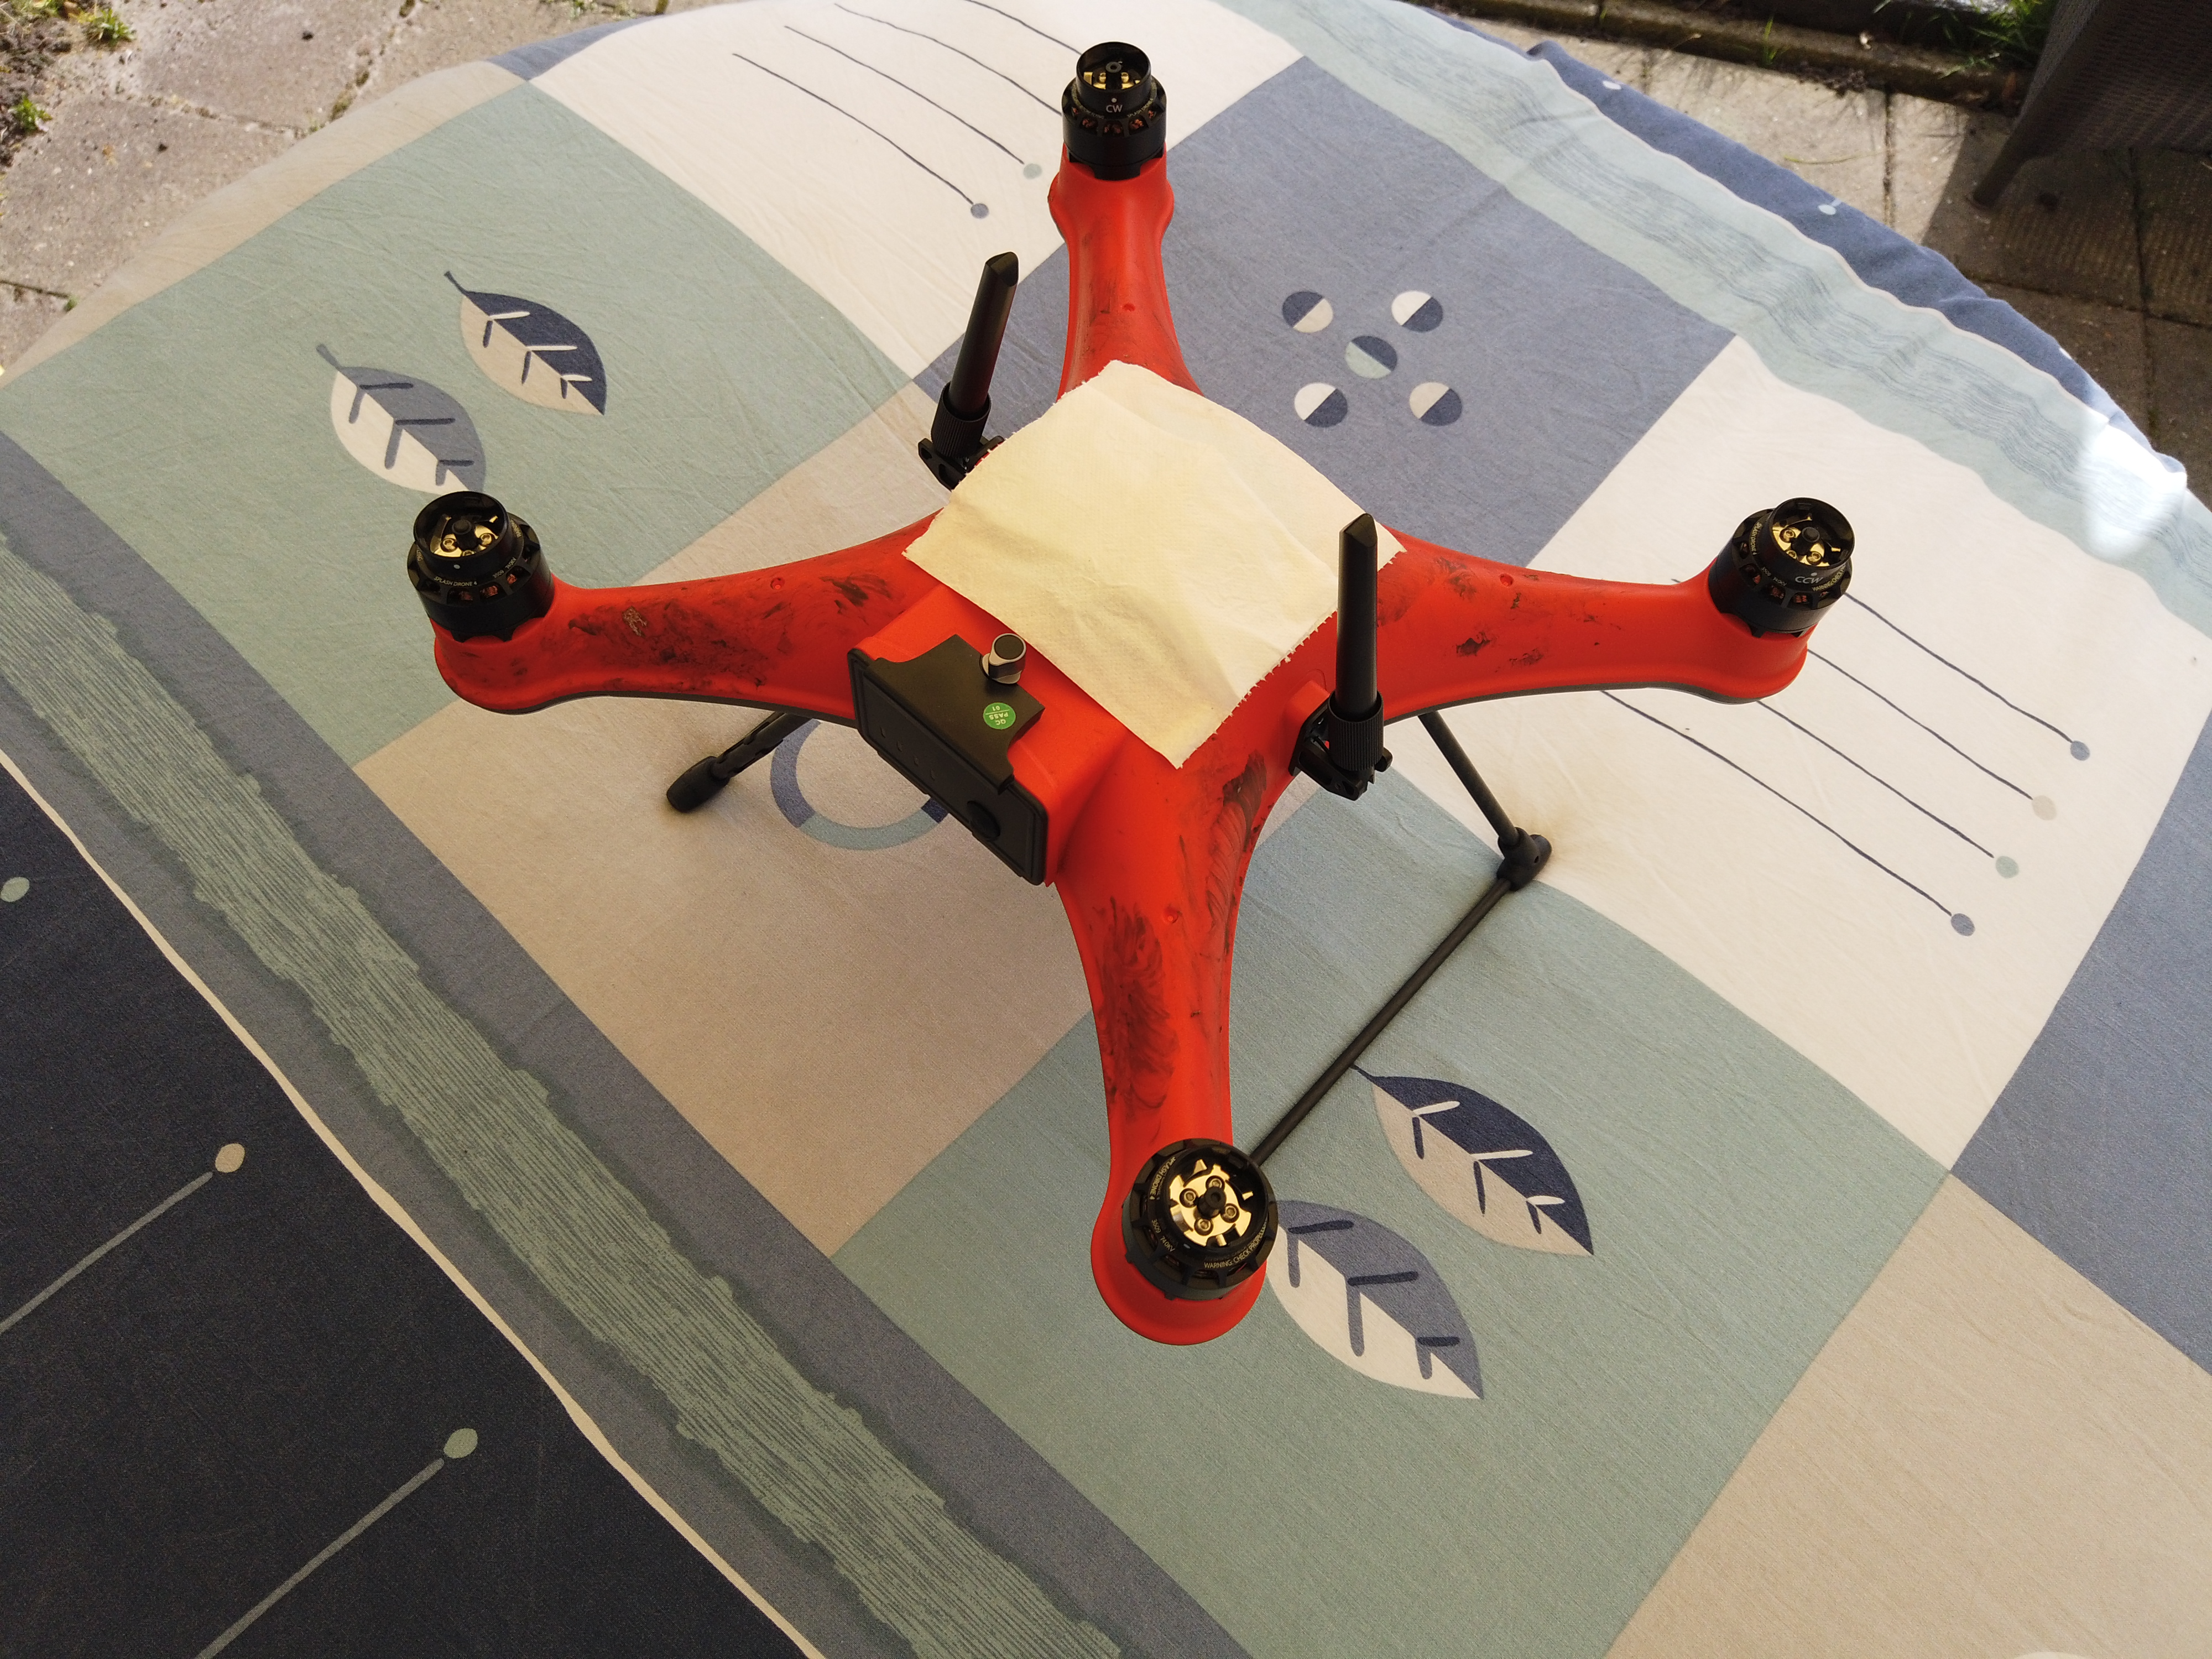
\includegraphics[width=\textwidth]{070_design/cadmodel/31_dphoto.jpg}
    \caption{Original photo \cite{dronemodel}}
  \end{minipage}
  \hfill
  \begin{minipage}[b]{0.5\textwidth}
    \includegraphics[width=\textwidth]{070_design/cadmodel/32_dmodel.png}
    \caption{3D Model \cite{dronemodel}}
  \end{minipage}
\end{figure}

The program failed to capture the gimbal of the drone accurately as it was able to move freely during capture. The bottom has been roughly reworked later on in \gls{CAD} software, leading to the following result:

\begin{figure}[h]
\centering
\includegraphics[scale=0.1]{070_design/cadmodel/33_dcadmodel.png}
\caption{Final CAD Model \cite{dronemodel}}
\end{figure}

As the gimbal of the drone is not of any importance, it is not modelled and instead modelled as a \gls{3D} box. While the model is not perfect, it is adequate for our use case.


\newpage
\subsection{Sensors}
After careful consideration, 4 water quality parameters are chosen to be monitored: turbidity, acidity, conductivity, and temperature. This set of sensors will help monitoring both the salinization issues and acidity issues at hand

\subsubsection{Turbidity}
To measure the turbidity, the DFRobot SEN0189 \cite{SEN0189} was chosen because of it's availability and ease of hooking up.
\begin{table}[h!]
	\centering
	\adjustimage{height=4cm,valign=c}{070_design/sensors/41_sen0189.jpg}\quad
	\begin{tabular}{| l | l |}
    \hline
    Protocol & Analog\\
    Operating Temperature & 5-90 ℃ \\
    Operating Range &  0-3000NTU\\
    Response time & Within 500ms \\
    Supply Voltage & 0V-4.5V \\
    Software library included & yes \\
    Availability & 3-5 Days \\
    \hline
	\end{tabular}
\end{table}

\subsubsection{Acidity}
To measure the acidity, the DFRobot SEN0169 V2 Pro \cite{SEN0169V2} was chosen because of it's ease of hooking up and existing software libraries.
\begin{table}[h!]
	\centering
	\adjustimage{height=4cm,valign=c}{070_design/sensors/42_gravityv2pro.jpg}\quad
	\begin{tabular}{| l | l |}
    \hline
    Interface & Analog \\
    Measurement Range & 0-14 pH \\
    Measurement Accuracy &  0.1pH \\
    Response time & Within 1\gls{min} \\
    Supply Voltage & 3.3V-5V \\
    Software library included & yes \\
    Long term immersion & yes \\
    Availability & 3-5 Working Days \\
    \hline
	\end{tabular}
\end{table}

\subsubsection{Conductivity}
To measure the conductivity, the DFRobot DFR0300H \cite{DFR0300H} was chosen because of its availability and included software library.
\begin{table}[h!]
	\centering
	\adjustimage{height=4cm,valign=c}{070_design/sensors/43_dfr0300h.jpg}\quad
	\begin{tabular}{| l | l |}
    \hline
    Protocol & Analog\\
    Measurement Accuracy &  5\% \gls{FSR}\\
    Supply Voltage & 3.3-5V\\
    Support Detection Range & 10~100ms/cm\\
    Software library included & yes \\
    Probe included & yes \\
    Availability & 3-5 Working days \\
    \hline
	\end{tabular}
\end{table}

\newpage
\subsubsection{Temperature}
To measure the temperature, the DFRobot DFR0198/DS18B20 \cite{DFR0198} was chosen because of the accuracy and fast response times.
\begin{table}[h!]
	\centering
	\adjustimage{height=4cm,valign=c}{070_design/sensors/44_dfr0198.jpg}\quad
	\begin{tabular}{| l | l |}
    \hline
    Protocol & 1-Wire\\
    Measurement Range & -10-85 ℃ \\
    Measurement Accuracy &  0.5 ℃ \\
    Response time & Within 750\gls{ms} \\
    Supply Voltage & 3.3V-5V \\
    Software library included & yes \\
    Availability & 3-5 Working Days \\
    \hline
	\end{tabular}
\end{table}

\subsubsection{MCU} \label{mcu}
An Arduino Uno derivative is used as the \gls{MCU} to power and log the sensors. The board  (Vietduino \cite{vietduino}) is based on the ATmega328P microcontroller, and has a CP2102 \gls{UART}-to-Serial interface. The Vietduino has superior power delivery over the original Arduino Uno. While a more performant MCU could have been used, an Arduino was chosen because of the popular form factor and the ease of rapid prototyping. The popularity of the board makes for an excellent base for people working on this project in the future.

\begin{figure}[h]
  \centering
  \begin{minipage}[b]{0.4\textwidth}
    \includegraphics[width=\textwidth]{070_design/sensors/45_vietduino.png}
    \caption{Vietduino \cite{vietduino}}
  \end{minipage}
  \hfill
  \begin{minipage}[b]{0.5\textwidth}
    \includegraphics[width=\textwidth]{070_design/sensors/46_screwshield.jpeg}
    \caption{Screw Shield V3 \cite{screwshield}}
  \end{minipage}
\end{figure}

A screw shield was used to help with cable management and rapid prototyping. This screw shield exposes the digital and analog pins on the Arduino alongside the ground and voltage rail. This way, there is no need for any breadboard.

To log the data locally on the device, a DS3231 RTC module and SD card adapter was used.

\newpage
\subsubsection{Schematics}
In the illustration below one can find the schematics of the sensors and the microcontroller board.
\begin{figure}[h]
\centering
\includegraphics[scale=0.8]{070_design/sensors/47_schematic.png}
\caption{MCU and sensors schematic}
\end{figure}


\newpage
\subsection{Sensor Package Design}
The sensors, the micro controller unit and the additional electronics are all combined in the sensor package. Throughout testing there has been revisions on this sensor package.\\

In the Preliminary Research Report it was stated that the project would make use out of \gls{3D} designs. As it turns out that the sensor package didn't require any unique shapes, it made better sense to edit existing enclosures, like project boxes.

\subsubsection{Revision 1}
The initial idea was to the components in one plastic enclosure. A project box was acquired at the Nhat Tao market and holes were drilled out at the side of the box to make mounts for the the turbidity, acidity, and conductivity sensors.

\begin{figure}[h]
\centering
\includegraphics[scale=0.1]{070_design/package/51_rev1.jpg}
\caption{Inside of the first revision}
\end{figure}

The bottom of the box has screw holes drilled out for mounting the \gls{PCB}s in the case. To prevent water from coming into the enclosure, O-rings are used along with sticky tack. Rubber inserts were used to close down the box. After some preliminary testing, it turned out that some water still leaked into the enclosure while fully submerged.
\newpage
\subsubsection{Revision 2}
On the second revision, a different approach was taken. The sensitive non-waterproof \gls{PCB}s were covered by a two-part epoxy, so that even if water would come into the enclosure, it would not be likely to short any circuits.\\

The \gls{PCB}s are mounted on a metal holed sheet covered with conductive tape. This way, the entire waterproof enclosure could be replaced easily in the future without dismounting any \gls{PCB}s. A swivel is used to lead the cables waterproof outside the enclosure. A battery bank is placed underneath the \gls{PCB}s for powering the electronics.

\begin{figure}[h]
  \centering
  \begin{minipage}[b]{0.4\textwidth}
    \includegraphics[width=\textwidth]{070_design/package/52_rev2.jpg}
    \caption{Inside of the second revision}
  \end{minipage}
  \hfill
  \begin{minipage}[b]{0.5\textwidth}
    \includegraphics[width=\textwidth]{070_design/package/53_mount.jpg}
    \caption{Full view of the drone}
  \end{minipage}
\end{figure}

The sensor probes are placed outside the enclosure on a rack underneath the drone to be fully submerged in the water, while the enclosure is placed on top of the drone above the water. The enclosure is slightly heightened so that the propellers of the drone can still move freely.\\

Throughout the drone, cable ties are used to fasten the enclosure, sensors and the rack. This is a very convenient and simple solution, as it allows one to quickly make changes to the design as the project goes forward, without investing a lot of time in a \gls{CAD} application. 

\newpage
\subsubsection{Secchi Disk}
To determine the turbidity, a secchi disk is used. This disk was made from an used 30\gls{cm} record. Tape was used to make the black and white sides. An eye bolt was used to make a hole for the rope to attach. The secchi disk is attached to the middle of the bottom grid of the drone.

\begin{figure}[h]
\centering
\includegraphics[scale=0.1]{070_design/package/54_secchi.jpg}
\caption{DIY Secchi Disk}
\end{figure}

A layer of transparent packing tape was used to cover the secchi disk to protect the colored tape. As seen in the photo, this introduces a lot of glare combined with the lighting. This may pose an issue when filming.
\newpage
\subsection{Software}
Throughout the project, software was developed to aid in the electronic logging of water quality parameters. In this section, an overview of these software projects will be given

\subsubsection{MCU Firmware}
As previously mentioned in \ref{mcu}, the Arduino environment was chosen to program the ATMega328P. The Arduino environment uses a C/C++ library which makes common input/output operations easier than writing the firmware "Bare-metal".\\

The firmware \cite{rwsuufirmware} is responsible for retrieving sensor values and logging them on a \gls{SD} card. Several libraries are used to aid in this process:

\begin{description}
   \item[DallasTemperature \cite{Dallas}] A library to read the temperature sensor
   \item[OneWire] \cite{OneWire} A library to access 1-Wire devices like the temperature sensor
   \item[DFRobot EC10] \cite{ec10} A library to read and calibrate the conductivity sensor
   \item[DFRobot PH] \cite{phlibrary} A library to read and calibrate the acidity sensor
   \item[DS1307RTC] \cite{DS1307RTC} A library to control the \gls{RTC} with the Time library
   \item[Time] \cite{timelibrary} A library for timekeeping functionality
   \item[SD] \cite{sdlibrary} A library for reading and writing to a SD card
\end{description}

Originally, the idea was to use CLion as the \gls{IDE}. As CLion is not well suited for Arduino development, PlatformIO \cite{platformio} is used in combination with VS Code instead as the \gls{IDE}. The code is still checked on MISRA standards using CLion. Documentation is generated from the source code via Doxygen. \cite{doxygen}
\newpage
\paragraph{SD Card} \label{sd}

The SD library is used to log the sensor values to the \gls{SD} card. An attempt was made to log the values in \gls{CSV} format to the \gls{SD} card, but string processing turned out to be quite resource intensive during testing. To save on resources, the decision was made to log the sensor values straight to a binary entry. Each binary entry has the following structure:

\begin{figure}[h]
\centering
\includegraphics[scale=0.45]{070_design/software/61_datastructure.png}
\caption{Data structure of binary file}
\end{figure}

A new .DAT file with an unique filename is created on each boot. Entries are placed next to each other in the file. A Golang\cite{golang} script has been made on the computer to convert the binary files to the desired \gls{CSV} format. \cite{dat2csv}

\paragraph{Sensors}

Every sensor has a simple and ordered interface interacting with the system:
\begin{enumerate}
  \item It has function that initializes the sensor that is called during the setup.
  \item It has a function that can calibrate the sensor. If necessary, it can be called at the end of the setup.
  \item It has a function that retrieves the value from the sensor that is called in the main loop
  \item It has an unique ID used when saving entries to the binary file.
\end{enumerate}

In the main loop, the sensor values are retrieved and stored on the \gls{SD} card.
\newpage
\subsubsection{Web Interface}
A web interface has been created using ThingsBoard \cite{thingsboard} to visualize the position of the drone and sensor data over time. This gives water quality researchers the tools to make sense of recorded data. Below, one can see the demo of the dashboard:

\begin{figure}[h]
\centering
\includegraphics[scale=0.3]{070_design/software/63_dashboard.png}
\caption{Dashboard}
\end{figure}

The communication of the sensor package and the drone is illustrated as follows:

\begin{figure}[h]
\centering
\includegraphics[scale=1]{070_design/software/62_comms.png}
\caption{Communication from sensor package to ThingsBoard}
\end{figure}

As one can see, the sensor package has a serial connection with the drone. The drone wirelessly passes through this serial connection to the remote controller. The data structure of the data passing through is the same as the data structure of each entry in the binary file on the SD Card, with a start bit added to indicate the beginning of the transmission. The remote controller has in turn a serial connection with the computer, and the computer is running a Golang script \cite{rwsuucontroller} to listen to this serial connection and pass this information to ThingsBoard.


\newpage
\section{Testing}
In this section, the designed prototypes will be tested on several quantitative and qualitative features. These features include accuracy, speed, and cost. This will be done by testing the prototypes both in the lab and in real world situations.

\begin{filecontents}{ph4.dat}
X Sample  	Hanna  DFRobot	
1 1         	4.4	4.3
2 2         	4.4	4.4
3 3         	4.4	4.4
4 4         	4.4	4.4
5 5         	4.4	4.4
\end{filecontents}

\begin{filecontents}{ph7.dat}
X Sample  	Hanna  DFRobot	
1 1         	7.2	7.3
2 2         	7.2	7.3
3 3         	7.2	7.3
4 4         	7.3	7.3
5 5         	7.2	7.3
\end{filecontents}

\begin{filecontents}{ec1288.dat}
X Sample  	DFRobot   Mean
1 1         	13.3   13.06
2 2         	13.0
3 3         	13.0
4 4         	12.9
5 5         	13.1   13.06
\end{filecontents}

\begin{filecontents}{ec1433.dat}
X Sample  	DFRobot   Mean
1 1         	1.6   1.56
2 2         	1.5
3 3         	1.6
4 4         	1.6
5 5         	1.5   1.56
\end{filecontents}

\begin{filecontents}{temp.dat}
X Sample  	Hanna  DFRobot	
1 1         	30.3 31.12
2 2         	30.4 31.44
3 3         	30.3 32.06
4 4         	30.5 32.13
5 5         	30.7 32.38
\end{filecontents}
\subsection{Sensors}

The sensor package on the drone is equipped with a turbidity, conductivity, and acidity meter. A minimum accuracy and range requirement for these sensors will be established based on an use case provided by PERNAM \gls{JSC}. Accuracy of these parameters will be measured both in the laboratory and in practice. All sensors are calibrated accordingly beforehand. A full morphological overview of the sensors can be found in the preliminary research report (Appendix A)

\subsubsection{Use case} \label{sensors:usecase}

PERNAM \gls{JSC} wishes to use an \gls{UAV} that has the capability to measure the turbidity, conductivity, and acidity around their water filtration plants in hopes to detect anomalies in the water input early on. For the system to be useful, they have listed some accuracy requirements as follows:

\begin{description}
   \item[Acidity] 2\% of full scale range so +/- 0.3pH
   \item[Conductivity] 5\% of full scale range so +/- 5ms/cm
   \item[Turbidity] 5\% of full scale range so +/- 150NTU
\end{description}

As seen in the tests below, the chosen sensors are accurate enough for PERNAM's use case.

\newpage
\subsubsection{Acidity} \label{sensors:acidity}

As mentioned in the Design Report, the DFRobot SEN0169 V2 Pro \cite{SEN0169V2} was chosen for measuring the acidity. The manufacturer claims the sensor has a resolution of 0.1pH across the whole range from 0 to 14pH.

\begin{figure}[h]
  \centering
  \begin{minipage}[b]{0.4\textwidth}
    \includegraphics[width=\textwidth]{080_testing/sensors/12_gravityv2pro.jpg}
    \caption{SEN0169 V2 Pro \cite{SEN0169V2}}
  \end{minipage}
  \hfill
  \begin{minipage}[b]{0.3\textwidth}
    \includegraphics[width=\textwidth]{080_testing/sensors/11_hanna.jpg}
    \caption{Hanna pHep \cite{hanna}}
  \end{minipage}
\end{figure}

The chosen sensor was compared against the Hanna pHep, that also has a resolution of 0.1pH. \cite{hanna} Two solutions with different pH were tested on both sensors. Before each sample was taken, both sensors were cleaned with distilled water. A sample is taken a minute after submersion, as the response time of both acidity sensors are within 1 minute.

\newpage
\paragraph{First solution}
The first solution is marked in pink.

\begin{figure}[h]
  \centering
  \begin{minipage}[b]{0.2\textwidth}
    \includegraphics[width=\textwidth]{080_testing/sensors/14_ph4_hanna.jpg}
    \caption{Hanna sensor measuring 4.4}
  \end{minipage}
  \hfill
  \begin{minipage}[b]{0.7\textwidth}
    \includegraphics[width=\textwidth]{080_testing/sensors/13_ph4_dfrobot.jpg}
    \caption{DFRobot sensor measuring 4.4}
  \end{minipage}
\end{figure}

\begin{figure}[h!]
\caption{Comparison between Hanna and DFRobot on pH 4.4}
\begin{tikzpicture}
\begin{axis}[
axis lines=middle,
ymin=0,
x label style={at={(current axis.right of origin)},anchor=north, below=10mm},
legend style={at={(0.7,0.7)},anchor=east},
ymin=4, ymax=5,
    xlabel=Samples,
  ylabel=pH,
   enlargelimits = true,
  xticklabels from table={ph4.dat}{Sample},xtick=data]
\addplot[orange,thick,mark=square*] table [y=Hanna,x=X]{ph4.dat};
\addlegendentry{Hanna}
\addplot[green,thick,mark=square*] table [y= DFRobot,x=X]{ph4.dat};
\addlegendentry{DFRobot}]
\end{axis}
\end{tikzpicture}
\end{figure}

As seen in the graph above, both sensors repeatedly measured a pH of 4.4. The DFRobot sensor read 4.3 on the first sample, this falls within the indicated margin of error.

\newpage
\paragraph{Second solution}
The second solution is marked in light yellow. The Hanna pHep repeatedly measured a pH of 7.2, while the DFRobot sensor repeatedly measured a pH of 7.3

\begin{figure}[h]
  \centering
  \begin{minipage}[b]{0.2\textwidth}
    \includegraphics[width=\textwidth]{080_testing/sensors/16_ph7_hanna.jpg}
    \caption{Hanna sensor measuring 7.2}
  \end{minipage}
  \hfill
  \begin{minipage}[b]{0.7\textwidth}
    \includegraphics[width=\textwidth]{080_testing/sensors/15_ph7_dfrobot.jpg}
    \caption{DFRobot sensor measuring 7.3}
  \end{minipage}
\end{figure}

\begin{figure}[h!]
\caption{Comparison between Hanna and DFRobot on pH 7.2}
\begin{tikzpicture}
\begin{axis}[
axis lines=middle,
ymin=0,
x label style={at={(current axis.right of origin)},anchor=north, below=10mm},
legend style={at={(0.7,0.7)},anchor=east},
ymin=7, ymax=8,
    xlabel=Samples,
  ylabel=pH,
   enlargelimits = true,
  xticklabels from table={ph4.dat}{Sample},xtick=data]
\addplot[orange,thick,mark=square*] table [y=Hanna,x=X]{ph7.dat};
\addlegendentry{Hanna}
\addplot[green,thick,mark=square*] table [y= DFRobot,x=X]{ph7.dat};
\addlegendentry{DFRobot}]
\end{axis}
\end{tikzpicture}
\end{figure}

As seen in the graph above, the Hanna sensor continously reads 7.2, while the DFRobot sensor continously reads 7.3. The exception is the fourth sample, when the Hanna sensor also read 7.2. This falls into the indicated margin of error.
\newpage
\subsubsection{Conductivity}
As mentioned in the Design Report, the DFRobot DFR0300H \cite{DFR0300H} was chosen for measuring the conductivity. The manufacturer claims the sensor has an accuracy of 5\% \gls{FSR}, meaning with a range of 20\gls{ms}/\gls{cm}, it has an error of 1\gls{ms}/\gls{cm}. Before each sample was taken, the sensor was cleaned with distilled water. A sample is taken a minute after submersion, as the response time of the conductivity sensors are within 1 minute.

\begin{table}[h!]
	\centering
	\adjustimage{height=4cm,valign=c}{080_testing/sensors/23_dfr0300h.jpg}\quad
	\begin{tabular}{| l | l |}
    \hline
    Protocol & Analog\\
    Measurement Accuracy &  5\% FSR\\
    Supply Voltage & 3.3-5V\\
    Support Detection Range & 10-100\gls{ms}/\gls{cm}\\
    Software library included & yes \\
    Probe included & yes \\
    Availability & 3-5 Working days \\
    \hline
	\end{tabular}
\end{table}

\paragraph{Known conductivity solutions}
Known conductivity solutions of 12.88\gls{ms}/\gls{cm} and 1.413\gls{ms}/\gls{cm} were used to determine the accuracy of the sensor. These known solutions come from the manufacturer of the sensor and were verified in their lab.

\newpage
\paragraph{First known conductivity solution}
The first solution has a known conductivity of 12.88\gls{ms}/\gls{cm}

\begin{figure}[h]
\centering
\includegraphics[scale=0.6]{080_testing/sensors/21_ec1288_dfrobot.jpg}
\caption{DFRobot sensor measuring 13.0\gls{ms}/\gls{cm} [own picture]}
\end{figure}

\begin{figure}[h!]
\caption{DFRobot 13.0\gls{ms}/\gls{cm} samples}
\begin{tikzpicture}
\begin{axis}[
axis lines=middle,
ymin=0,
x label style={at={(current axis.right of origin)},anchor=north, below=10mm},
legend style={at={(0.7,0.7)},anchor=east},
ymin=12, ymax=14,
    xlabel=Samples,
  ylabel=ms/cm,
   enlargelimits = true,
  xticklabels from table={ec1288.dat}{Sample},xtick=data]
\addplot[green,thick,mark=square*] table [y= DFRobot,x=X]{ec1288.dat};
\addlegendentry{DFRobot}]
\addplot[red] table [y= Mean,x=X]{ec1288.dat};
\addlegendentry{mean}]
\end{axis}
\end{tikzpicture}
\end{figure}

As seen in the graph above, all samples fall well within the error range of 1\gls{ms}/\gls{cm}. The mean of the samples are 13.06\gls{ms}/\gls{cm}. The sensor performed better than advertised.

\newpage
\paragraph{Second known conductivity solution}
The second solution has a known conductivity of 1.413\gls{ms}/\gls{cm}

\begin{figure}[h]
\centering
\includegraphics[scale=0.6]{080_testing/sensors/22_ec1413_dfrobot.jpg}
\caption{DFRobot sensor measuring 1.6\gls{ms}/\gls{cm} [own picture]}
\end{figure}

\begin{figure}[h!]
\caption{DFRobot 1.413\gls{ms}/\gls{cm} samples}
\begin{tikzpicture}
\begin{axis}[
axis lines=middle,
ymin=0,
x label style={at={(current axis.right of origin)},anchor=north, below=10mm},
legend style={at={(0.7,0.1)},anchor=east},
ymin=1.4, ymax=1.7,
    xlabel=Samples,
  ylabel=ms/cm,
   enlargelimits = true,
  xticklabels from table={ec1433.dat}{Sample},xtick=data]
\addplot[green,thick,mark=square*] table [y= DFRobot,x=X]{ec1433.dat};
\addlegendentry{DFRobot}]
\addplot[red] table [y= Mean,x=X]{ec1433.dat};
\addlegendentry{mean}]
\end{axis}
\end{tikzpicture}
\end{figure}

As seen in the graph above, all samples fall well within the error range of 1\gls{ms}/\gls{cm}. The mean of the samples are 1.56\gls{ms}/\gls{cm}. The sensor performed better than advertised.
\newpage
\subsubsection{Temperature}
As mentioned in the Design Report, the DFRobot DFR0198/DS18B20 \cite{DFR0198} waterproof sensor was chosen to measure the temperature. Temperature readings of the water are both recorded and used to help determining the acidity and conductivity.

\begin{table}[h!]
	\centering
	\adjustimage{height=4cm,valign=c}{080_testing/sensors/31_dfr0198.jpg}\quad
	\begin{tabular}{| l | l |}
    \hline
    Protocol & 1-Wire\\
    Measurement Range & -10-85 ℃ \\
    Measurement Accuracy &  0.5 ℃ \\
    Response time & Within 750ms \\
    Supply Voltage & 3.3V-5V \\
    Software library included & yes \\
    Availability & 3-5 Working Days \\
    \hline
	\end{tabular}
\end{table}

Temperature readings are compared from the Hanna pH sensor and the DFRobot DS18B20 sensor. The Hanna sensor has an accuracy of 1℃ and the DFRobot sensor has an accuracy of 0.5 ℃  The results can be seen in the graph below.

\begin{figure}[h!]
\caption{Comparison between Hanna and DFRobot}
\begin{tikzpicture}
\begin{axis}[
axis lines=middle,
ymin=0,
x label style={at={(current axis.right of origin)},anchor=north, below=10mm},
legend style={at={(1,0.1)},anchor=east},
ymin=29, ymax=33,
    xlabel=Samples,
  ylabel=°C,
   enlargelimits = true,
  xticklabels from table={temp.dat}{Sample},xtick=data]
\addplot[orange,thick,mark=square*] table [y=Hanna,x=X]{temp.dat};
\addlegendentry{Hanna}
\addplot[green,thick,mark=square*] table [y= DFRobot,x=X]{temp.dat};
\addlegendentry{DFRobot}]
\end{axis}
\end{tikzpicture}
\end{figure}

As seen in the graph above, all samples could fall within both error ranges. As the Hanna sensor has a temperature accuracy of only 1℃ it is not possible to determine whether the DFRobot sensor is acting
\newpage
\subsection{Flights}
Throughout the projects, several flights have been performed to test the functionality of the drone and the prototypes.

\subsubsection{Flight Report: After calibration}
\begin{minipage}{1\textwidth}
	\begin{flushright}
		Date: 19-04-2022\\
		Location: Ton Duc Thang University\\
		Coordinates: 10.731373, 106.695396\\
		Flight Mode: \gls{GPS}\\
		Flight Duration: 30 minutes\\\vspace{5mm}
	\end{flushright}
\end{minipage}

The goal of this flight was to check if the drone was in fully working order after the trip to Vietnam. The drone was updated to the latest available firmware. The drone's compass, the gyroscope, and the \gls{IMU} was fully calibrated using the instructions in the user manual. \cite{splashdronemanual} The calibration itself turned out to be a challenge as a level surface was required, and this was not directly available at the testing site.\\

After finding a level surface and calibrating the drone however, it flew without any issues. The drone was able to land and take off in the water. \\

As the drone had to land in the water, the drone's antennas were place in an upward position for it to have signal. This means the maximum altitude without signal problems was noticeably reduced.


\newpage
\subsubsection{Flight Report: Mount Stability}
\begin{minipage}{1\textwidth}
	\begin{flushright}
		Date: 29-05-2022\\
		Location: Near Sunrise Riverside Block K\\
		Coordinates: 10.724144, 106.704113\\
		Flight Mode: \gls{GPS}\\
		Flight Duration: 15 minutes\\\vspace{5mm}
	\end{flushright}
\end{minipage}

The goal of this flight was to check if the drone was stable when flying with the second revision of the sensor package as described in the Design Report. \cite{designreport}

\begin{figure}[h]
\centering
\includegraphics[scale=0.4]{080_testing/flights/21_drone.jpg}
\caption{Drone with the second revision of the sensor package [own picture]}
\end{figure}

The drone flew for 15 minutes around a grass field at different speeds and altitudes. In the following sections, potential risks will be elaborated and evaluated based on this test flight.

\paragraph{The center of mass could be shifted too much}
Due to the sensor placement on the bottom of the drone, the center of mass could be shifted too much, causing drift to one direction. During this test flight, I did not experience such a thing. The drone did not drift to any direction during the whole flight.\\

While changing directions, I did notice the drone took some more space and time to stabilize its position.

\paragraph{The drone could be too heavy}
Due to the weight of the sensor package, the drone might not be able to take off or remain a stable altitude during flight. During this test flight, I noticed that the drone took far more force to take off. The drone needed manual assistance with the remote control to remain the same altitude.

\paragraph{The sensor package could not be stable enough}
Due to the mounting solution, the electronics enclosure and the sensors could move or fall off during flight. During this test flight, this did not happen. The enclosure and sensors were not moving

\paragraph{The sensor is blocking the view of the camera}
Due to the mounting solution, the electronics enclosure and the sensors could move or fall off during flight. During this test flight, this did not happen. The enclosure and sensors seemed stable, even when moving the drone at fast speeds

\paragraph{The electronics enclosure could block the propellers}
The electronics enclosure could not make it possible for the propellers move freely during flight, this could result in a crash. During this test flight, this did not happen. There was ample space for the propellers to move freely, even when moving the drone at fast speeds

\paragraph{Conclusion}
While manual intervention is sometimes necessary, I feel comfortable enough to perform a full test flight in the water.
\newpage
\subsubsection{Flight Report: Sensor Test}
\begin{minipage}{1\textwidth}
	\begin{flushright}
		Date: 30-05-2022\\
		Location: Hoa Phu Pump Station\\
		Coordinates: 10.9854687, 106.6186905\\
		Flight Mode: \gls{GPS}\\
		Flight Duration: 25 minutes\\\vspace{5mm}
	\end{flushright}
\end{minipage}

The goal of this flight was to fully test the second revision of the sensor package. The flight took place at the Hoa Phu Pump Station partially managed by PERNAM. A small presentation of the project goal was given before the test flight.

\begin{figure}[h]
\centering
\includegraphics[scale=1.2]{080_testing/flights/32_explanation.jpg}
\caption{A small presentation about the project}
\end{figure}

The drone seemed stable when gaining altitude. When the drone was above the water however, I noticed that it started slightly drifting away from the test site. An emergency landing had to be made, so there were several options.


One could land in the water. This was however a bit risky due to the fact that landing in the water while moving causes the drone to flip. While flipping over in the water is not an issue in normal operation of the drone, it was not clear what would happen with the sensor package. The water also had flow, so if the drone would be uncontrollable, we had to retrieve it while moving in the water.\\

I opted to bring the drone back to land so that retrieval of the drone was possible. The drone has a built in back to home function, but this did not work like intended. The drone went in the other direction, so I opted to land the drone at the other side of the land.
\newpage

\begin{figure}[h]
\centering
\includegraphics[scale=1.2]{080_testing/flights/31_flight.jpg}
\caption{The flight route of the drone}
\end{figure}

This land unfortunately had high grass, so the drone did not land gracefully. Retrieving the drone was done by going to the coordinates of the remote controller. This involved a motorbike ride of 20 minutes. When I got there, the drone had 1 damaged motor and minor damage to the landing gears.

\begin{figure}[h]
\centering
\includegraphics[scale=1]{080_testing/flights/33_afterflight.jpg}
\caption{Retrieving the drone after the crash}
\end{figure}

\paragraph{The cause}
There could be multiple reasons why the drone reacted the way it did during the flight. The most logical explanation would be that the calibration of the drone, combined with the slight imperfections seen at the center of mass caused the drone to drift. Return-to-home may not have worked because of poor \gls{GPS} reception at the test site.

\paragraph{Improvements}
Drift would not be such an issue if the weight of the sensor enclosure would be less. Custom casing could be designed that could fit the components better.
\newpage
\section{Conclusion}
The purpose of this project was to find out what the best way is to build a mobile surface water quality sensoring system that can take samples in remote areas. Based on the preliminary research, design, and testing that has been done during this project, it can be concluded that there are multiple options for such a system to be realized. \\

The electronic sensors used were accurate enough to prove useful in a real use case. Furthermore, the software that has been written proved to be working as expected and up to standards. It turns out it is possible to make a remote water sensing system using drones from a software perspective.\\

The sensor package leaves much to be desired from a design standpoint. From testing, it turned out that the drone with sensor package is too unstable to perform any measurements at this point in time. 

As seen, turbidity measurements with a secchi disk turns out to have potential, though the weight of such a disk causes the drone to use more power, which in turn reduces the battery life, limiting real implementations.

With the multidisciplinary research that has been done, it can be concluded that an improvement of the current sensor package design would be the best way to build a mobile surface water quality sensoring system that can take samples in remote areas. While a minimum viable product wasn't realized, the project did succeed to adhere to the rest of the MoSCoW prioritizations.

\subsection{Recommendations}
This project has come a long way in realizing a remote water sensing solution using drones. There are a few things that still need to be done to make this project a success.\\

A recommendation is to decrease the size and weight of the sensor package. An electronics engineering student could work on creating a custom printed circuit board, and a mechatronics student could for example work on designing a more permanent mounting solution. More care has to be put into the mounting location of the sensor package, so that it does not block the compass.\\

If the drone is stable enough, one could start to work on some automation by controlling the drone via the flight control communication protocol \cite{splashdronemanual} rather than the app. If this is a success, machine vision could be used as a way to automate secchi disk measurements and to detect anomalies in the water.\\

During this project, near infrared cameras as mentioned in the preliminary research report weren't realized as there was a lack of time to really do this subject with the attention it deserves. A recommendation is to reconsider it as an alternative option to take remote samples.

\newpage
\printbibliography
\newpage
\section{Appendix A: Preliminary Research Report}

\end{document}